%\documentclass[handout]{beamer}
\documentclass{beamer}
\usepackage[normalem]{ulem}
\usepackage{amssymb}
\usepackage{pifont}
%\definecolor{links}{HTML}{2A1B81}
%\definecolor{links}{HTML}{A80000}
\definecolor{links}{HTML}{006600}
\definecolor{zod}{HTML}{006600}
\hypersetup{colorlinks,linkcolor=,urlcolor=links}
%\usetheme{Goettingen}

\title{Sonar}
\author{Mate Lakat}

\setbeamertemplate{footline}[text line]{
    \parbox{\linewidth}{
        \vspace*{-8pt}
        \href{http://www.sonarqube.org/}{Sonar}
        \hfill
        \insertshortauthor
        \hfill
        \insertpagenumber
    }
}

\newcommand{\tick}{{\color{zod}{\ding{52}}}}
\newcommand{\cross}{\ding{56}}
\newcommand{\myhref}[2]{\href{#1}{{\uline{#2}}}}
\newcommand{\myttt}[1]{\colorbox{yellow}{#1}}

\setbeamertemplate{navigation symbols}{}
\date{2014-06-02}

\begin{document}

\begin{frame}
    \titlepage
\end{frame}

\begin{frame}
    \frametitle{Introduction}
    \begin{itemize}
        \item Jenkins
        \pause
        \begin{itemize}
            \item Build
            \pause
            \item Run tests
            \pause
            \item Run tools
            \pause
            \item Display results
            \pause
        \end{itemize}
    \end{itemize}

    \resizebox{\textwidth}{!}{
    
\includegraphics{so-what.jpeg}}
\end{frame}

\begin{frame}
    \frametitle{Meet Sonar}
    \begin{block}{What is Sonar?}
    Sonar is an open source quality management platform, dedicated to
    continuously analyze and measure technical quality, from project portfolio
    to method.
    \end{block}

    \pause
    \begin{itemize}
        \item Display results over time
        \pause
        \item Convert results to issues (instead of meaningless numbers)
        \pause
        \item Framework to fix the issues in a controlled way
        \pause
        \item Quality gate
            \pause
            \begin{itemize}
                \item New code is covered with tests
                \item New code doesn't contain violations
            \end{itemize}
    \end{itemize}
\end{frame}

\begin{frame}
    \frametitle{Components of Sonar}
    \resizebox{\textwidth}{!}{
    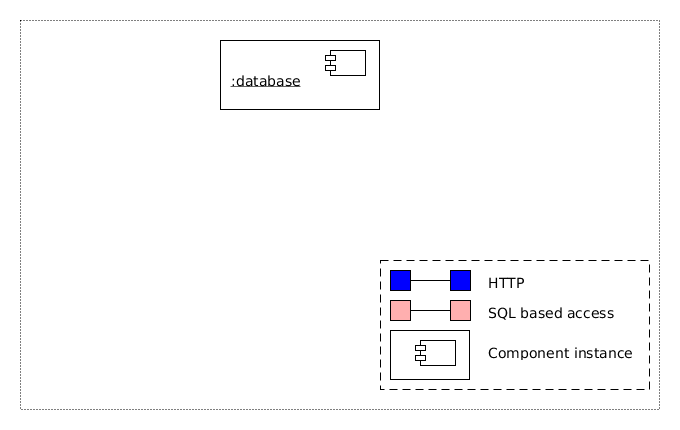
\includegraphics{sonar_components_1.png}}
\end{frame}

\begin{frame}
    \frametitle{Components of Sonar}
    \resizebox{\textwidth}{!}{
    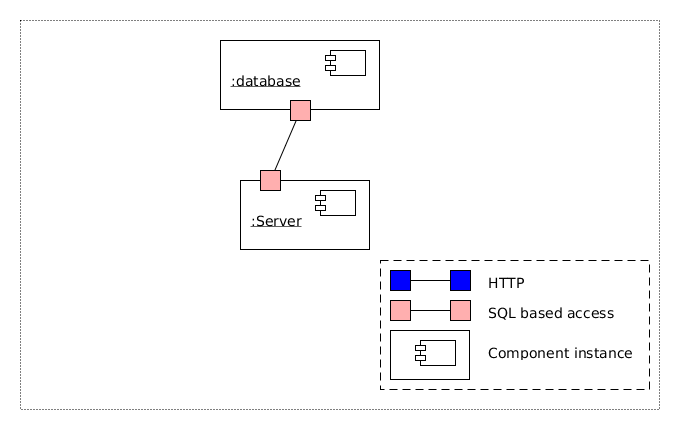
\includegraphics{sonar_components_2.png}}
\end{frame}

\begin{frame}
    \frametitle{Components of Sonar}
    \resizebox{\textwidth}{!}{
    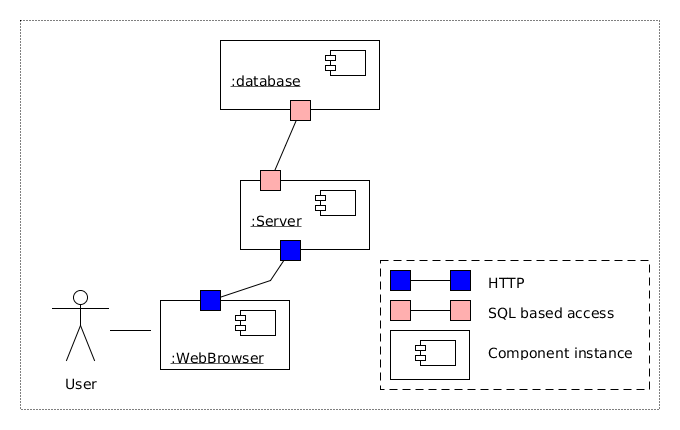
\includegraphics{sonar_components_3.png}}
\end{frame}

\begin{frame}
    \frametitle{Components of Sonar}
    \resizebox{\textwidth}{!}{
    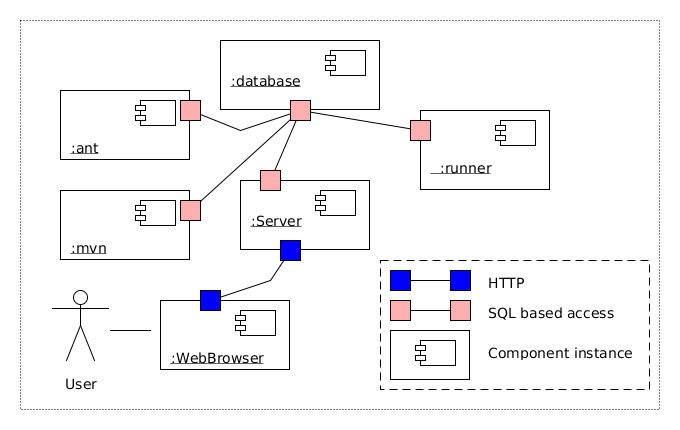
\includegraphics{sonar_components_4.png}}
\end{frame}

\begin{frame}
    \frametitle{Components of Sonar}
    \resizebox{\textwidth}{!}{
    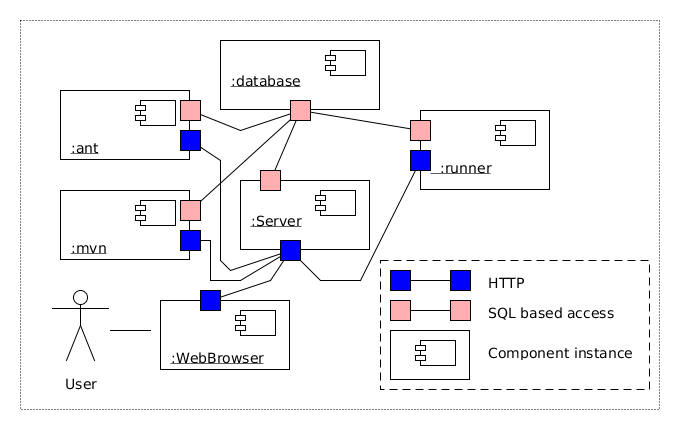
\includegraphics{sonar_components_5.png}}
\end{frame}

\begin{frame}
    \frametitle{The Analyzer (mvn/ant/standalone)}
    \begin{itemize}
        \item Analyze the code
        \pause
        \item Upload the results
        \pause
        \item Upload other tool's results (coverage)
        \pause
        \item Analysis/Preview/Incremental:
        \begin{itemize}
            \item[analysis] Analyse the code and upload the results (daily)
            \item[preview] Analyse without upload (CI)
            \item[incremental] Any new issues introduced?
        \end{itemize}
    \end{itemize}
\end{frame}

\begin{frame}
    \frametitle{The Server}
    \begin{itemize}
        \item Display Metrics
        \pause
        \item Drilldown issues
        \pause
        \item Create plans
        \pause
        \item Setup a quality gate
    \end{itemize}
\end{frame}

\begin{frame}
    \begin{center}
        \Large{Demo}
    \end{center}
    \begin{block}{}
    \begin{itemize}
    \pause
    \item Create a new project
    \pause
    \item Disable some violations
    \pause
    \item Setup a Quality Gate
    \end{itemize}
    \end{block}
\end{frame}

\begin{frame}
\frametitle{Notes}
\begin{block}{I learned them the hard way...}
\begin{itemize}
    \item Pylint: you have to enable pylint violations in your profile
    \item Pylint: use a version that recognises \texttt{-f parseable}
    \item nose, coverage: had to \texttt{sed} the results for full paths -
    otherwise they were not found
    \item Build breaker: enable in preview mode - settings/general/Plugins
    accepted for Preview and Incremental modes := \texttt{buildbreaker}
    \item coverage on new code: Install SCM plugin
    \item everything is on \myhref{https://github.com/matelakat/sonar-investigation}{github.com/matelakat/sonar-investigation}
\end{itemize}
\end{block}
\end{frame}


\begin{frame}
    \begin{center}
        \Large{The End}
    \end{center}
\end{frame}

\end{document}
